\chapter{業務用オーディオの利用現場と関連技術}
\label{chap:related_works}

本章では、業務用オーディオが利用されている現場とそれらを取り巻く周辺環境、運用上の課題について解説する。

\section{構成}

業務用オーディオが利用されている現場は、町の小規模な祭りからイベント、ライブやコンサートなど多岐にわたる。本項では、同時に複数人がマイクを利用するトークイベントを例に、実際の現場で利用されている構成を紐解いていく。

オーディオの伝送経路にアナログ伝送を用いた、非常に簡素な構成を図\ref{fig:pa_equipment_analog}に示す。オーディオの入力から出力まで数多くの機器が存在するケースもあるが、接続図では省略する。

\begin{figure}[htbp]
  \centering
  \label{fig:pa_equipment_analog}
  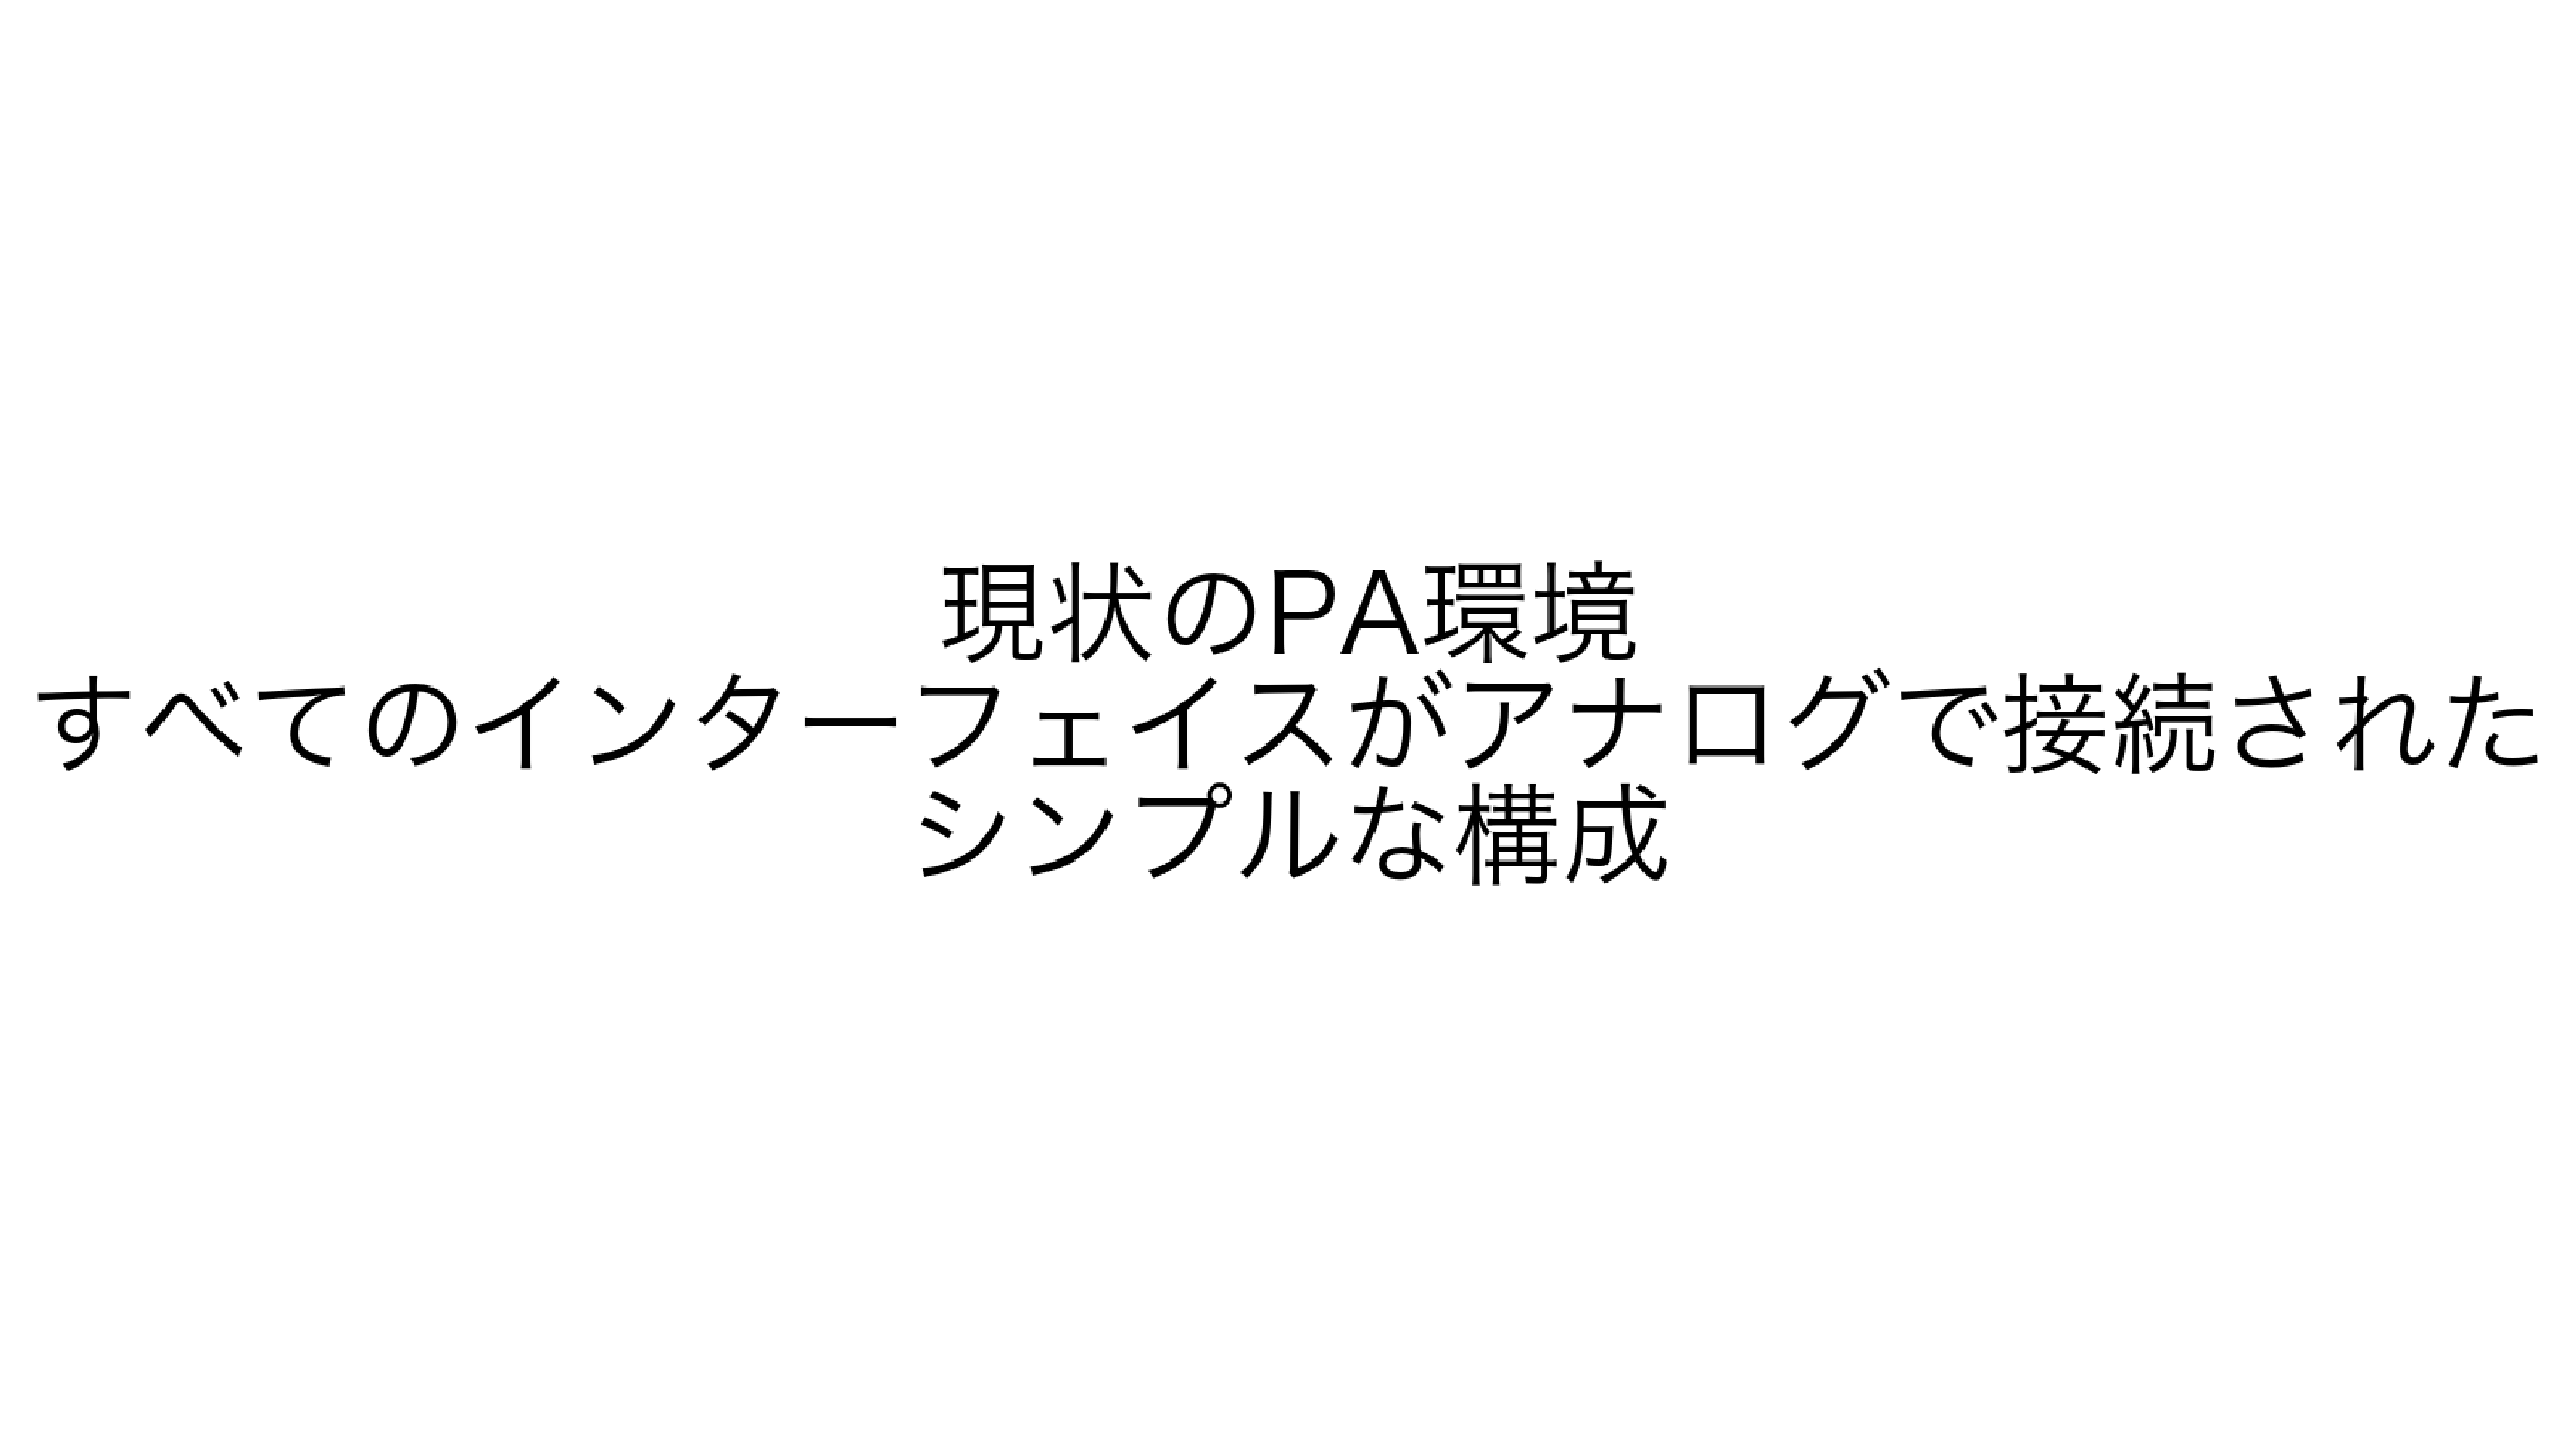
\includegraphics[width=0.8\linewidth]{img/pa_equipment_analog.pdf}
  \caption{アナログ伝送を使用した接続図}
\end{figure}

4本のマイクを1台のミキサーに入力し、複数のソースのオーディオをミックスしたオーディオが出力される。この構成では、すべての伝送経路をアナログ伝送によって行われている。アナログ伝送の場合、原則オーディオ1チャンネル\footnote{オーディオ信号の入出力の数。マイクの場合、1本につき1チャンネル。スピーカーが一般的なステレオ構成であれば2チャンネルとなる。}につきケーブルが1本ずつ必要となる。

次に、IPベースのデジタル伝送を用いた場合オーディオ機器同士の接続は、図\ref{fig:pa_equipment_digital}のように変化する。

\begin{figure}[htbp]
  \centering
  \label{fig:pa_equipment_digital}
  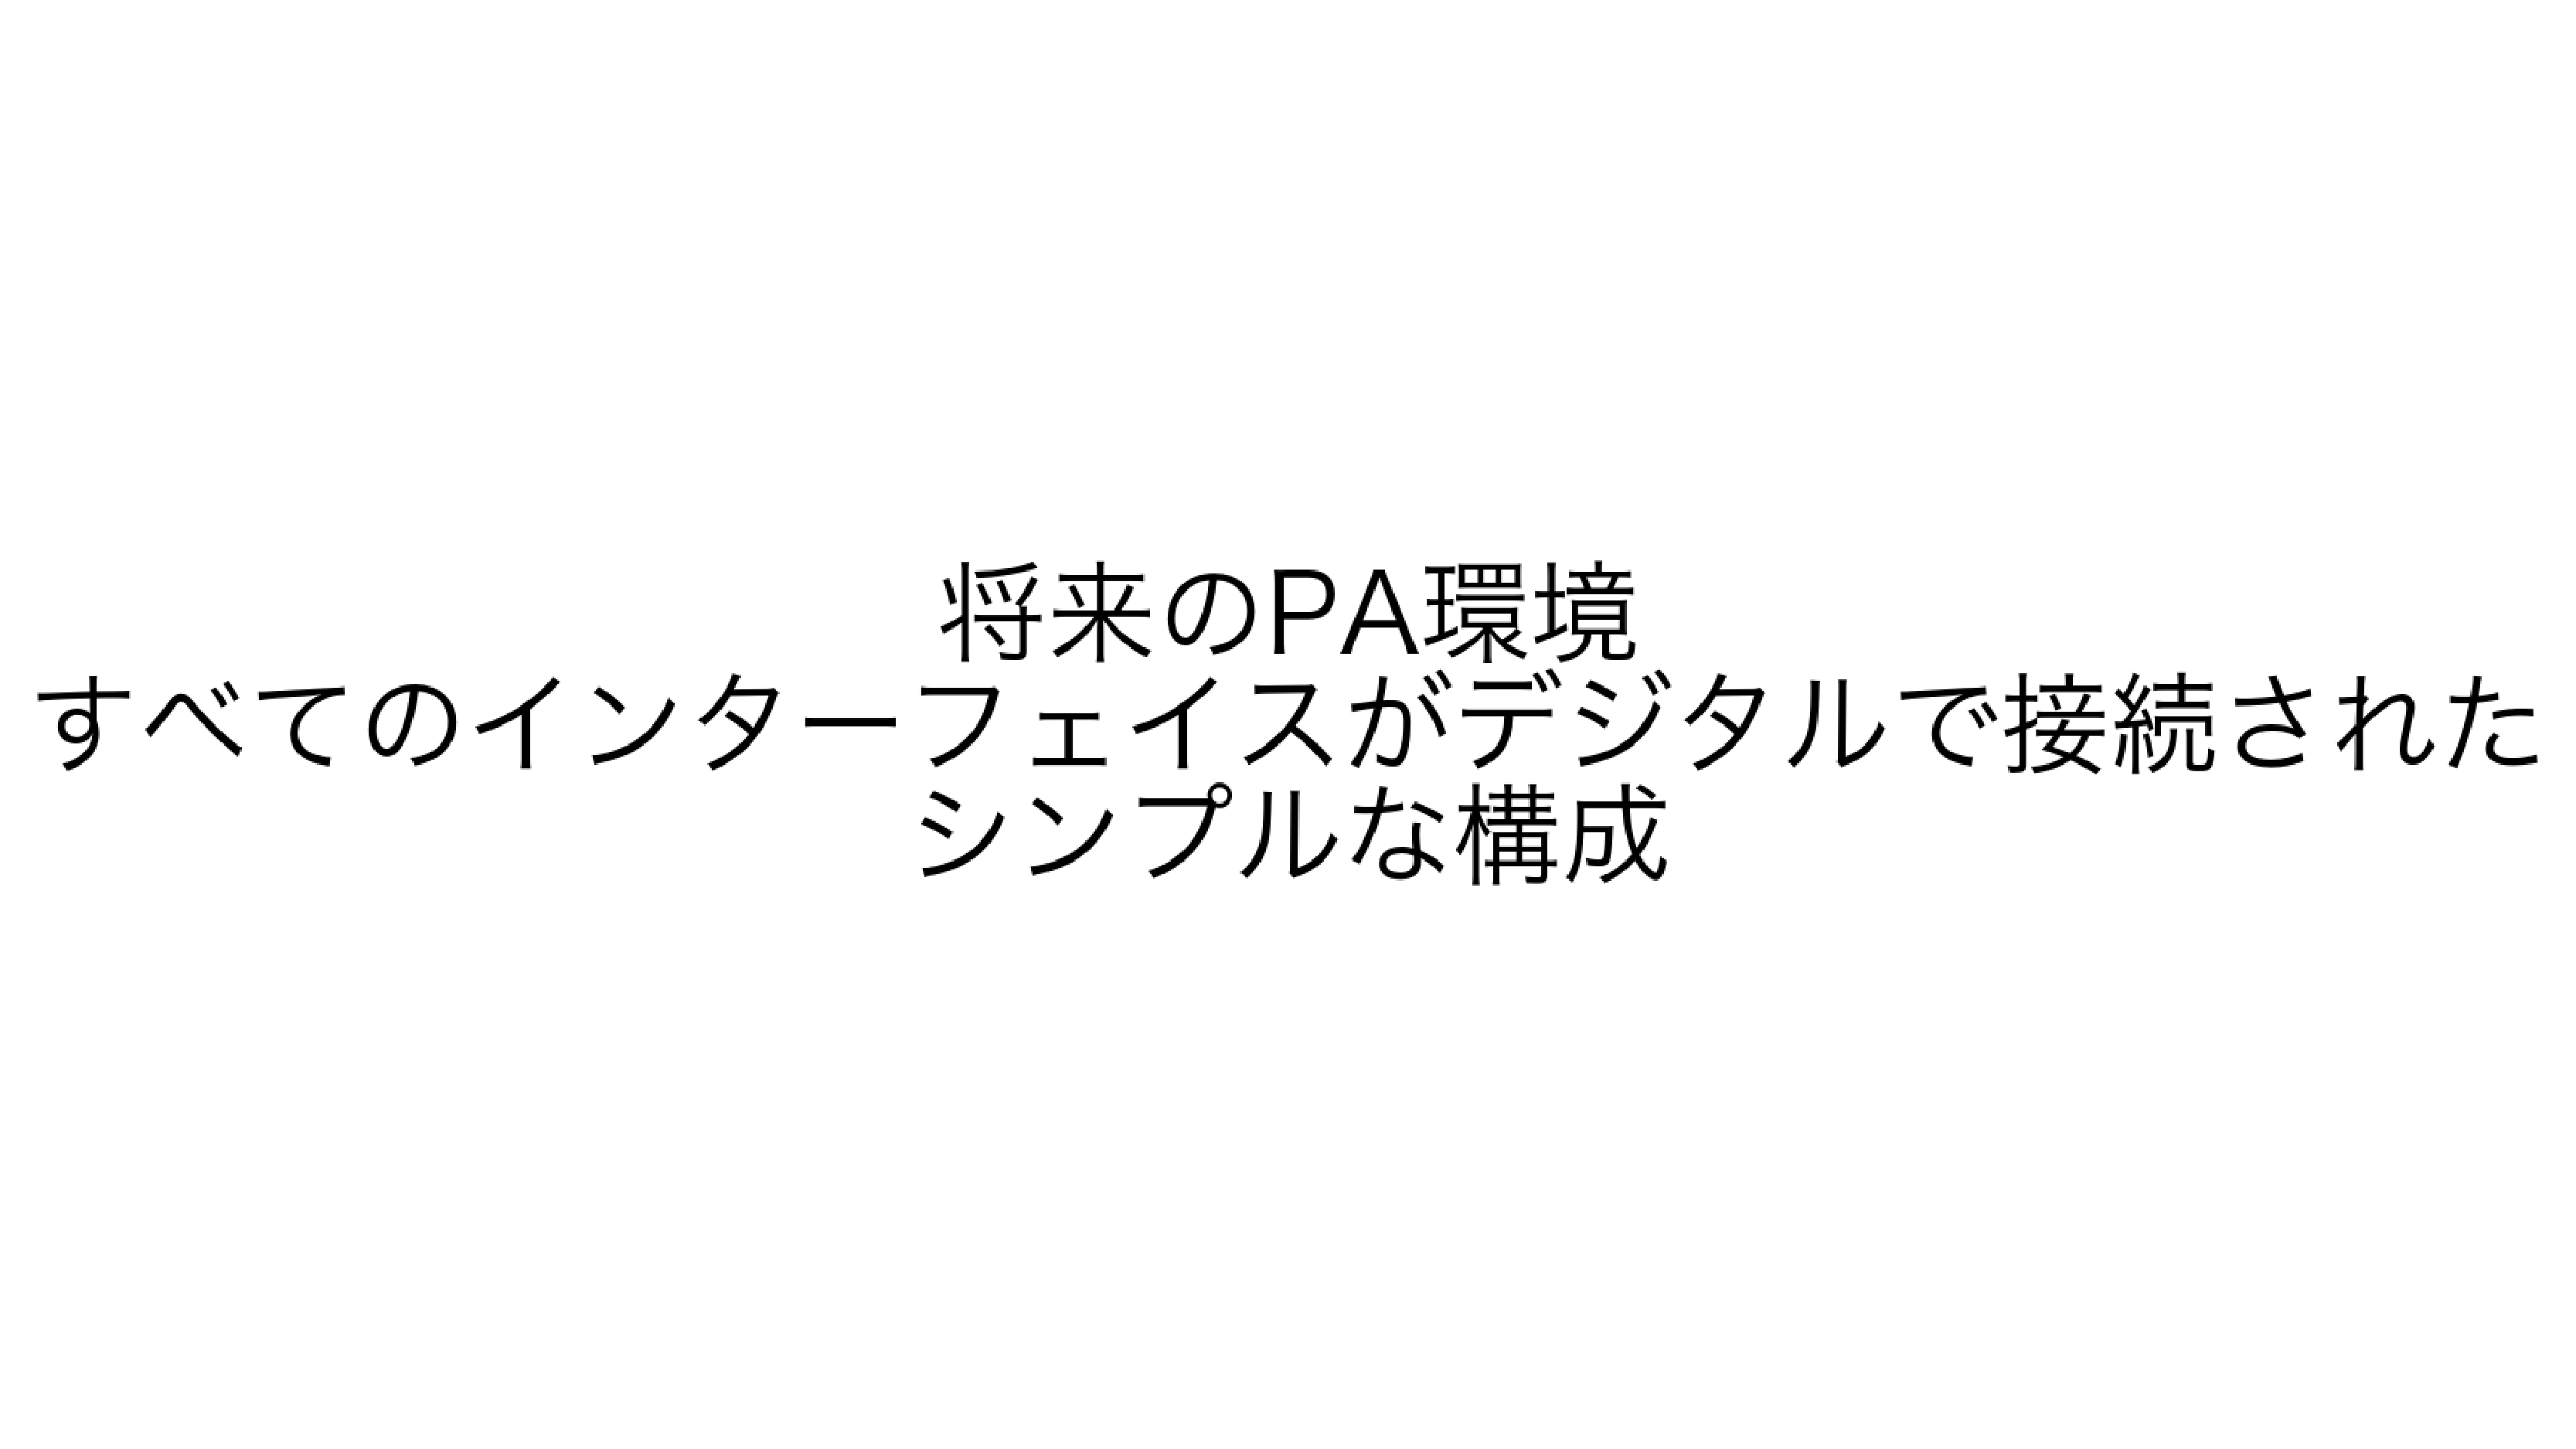
\includegraphics[width=0.8\linewidth]{img/pa_equipment_digital.pdf}
  \caption{デジタル伝送を使用した接続図}
\end{figure}

IPベースのデジタル伝送では、すべての伝送をL2スイッチを介して行う。コンピュータ同士を接続するネットワークに用いる汎用的な製品で対応できるため、同時にオーディオ以外のデータの送受信も可能だ。アナログ伝送では、オーディオ1チャンネルあたりにケーブル1本が必要となるため、ステレオの伝送に2本必要としていた。一方デジタル伝送では、多チャンネル伝送ができるためケーブルは1本で送信することができる。

\section{オーディオ機器}

本節では、図\ref{fig:pa_equipment_analog}と図\ref{fig:pa_equipment_digital}で示したオーディオ機器について、解説する。

\subsection{マイク}

マイクは、音声を電気信号に変換する装置である。伝送方式から、有線マイクと無線マイク(以下、ワイヤレスマイク)に分類できる。

ワイヤレスマイクの場合、送信機と受信機に分かれている。送信機は、マイクで変換した信号をアンテナを通して無線によって伝送する。受信機は、アンテナから受信した電波という構成だ。それらを総称してワイヤレスシステムと呼ばれることがある。

\begin{figure}[htbp]
  \centering
  
\includegraphics[width=0.4\linewidth]{img/microphone.pdf}
  \caption{マイク}
\end{figure}

\subsection{ミキサー}

ミキサーは、複数チャンネルのオーディオ入力をミックスし、1チャンネル以上の出力をする装置である。アナログミキサーとデジタルミキサーの2つに分類できる。ミックス処理をアナログ回路で行うか、DSP\footnote{Digital Signal Processor}によって行うかの違いがある。

\begin{figure}[htbp]
  \centering
  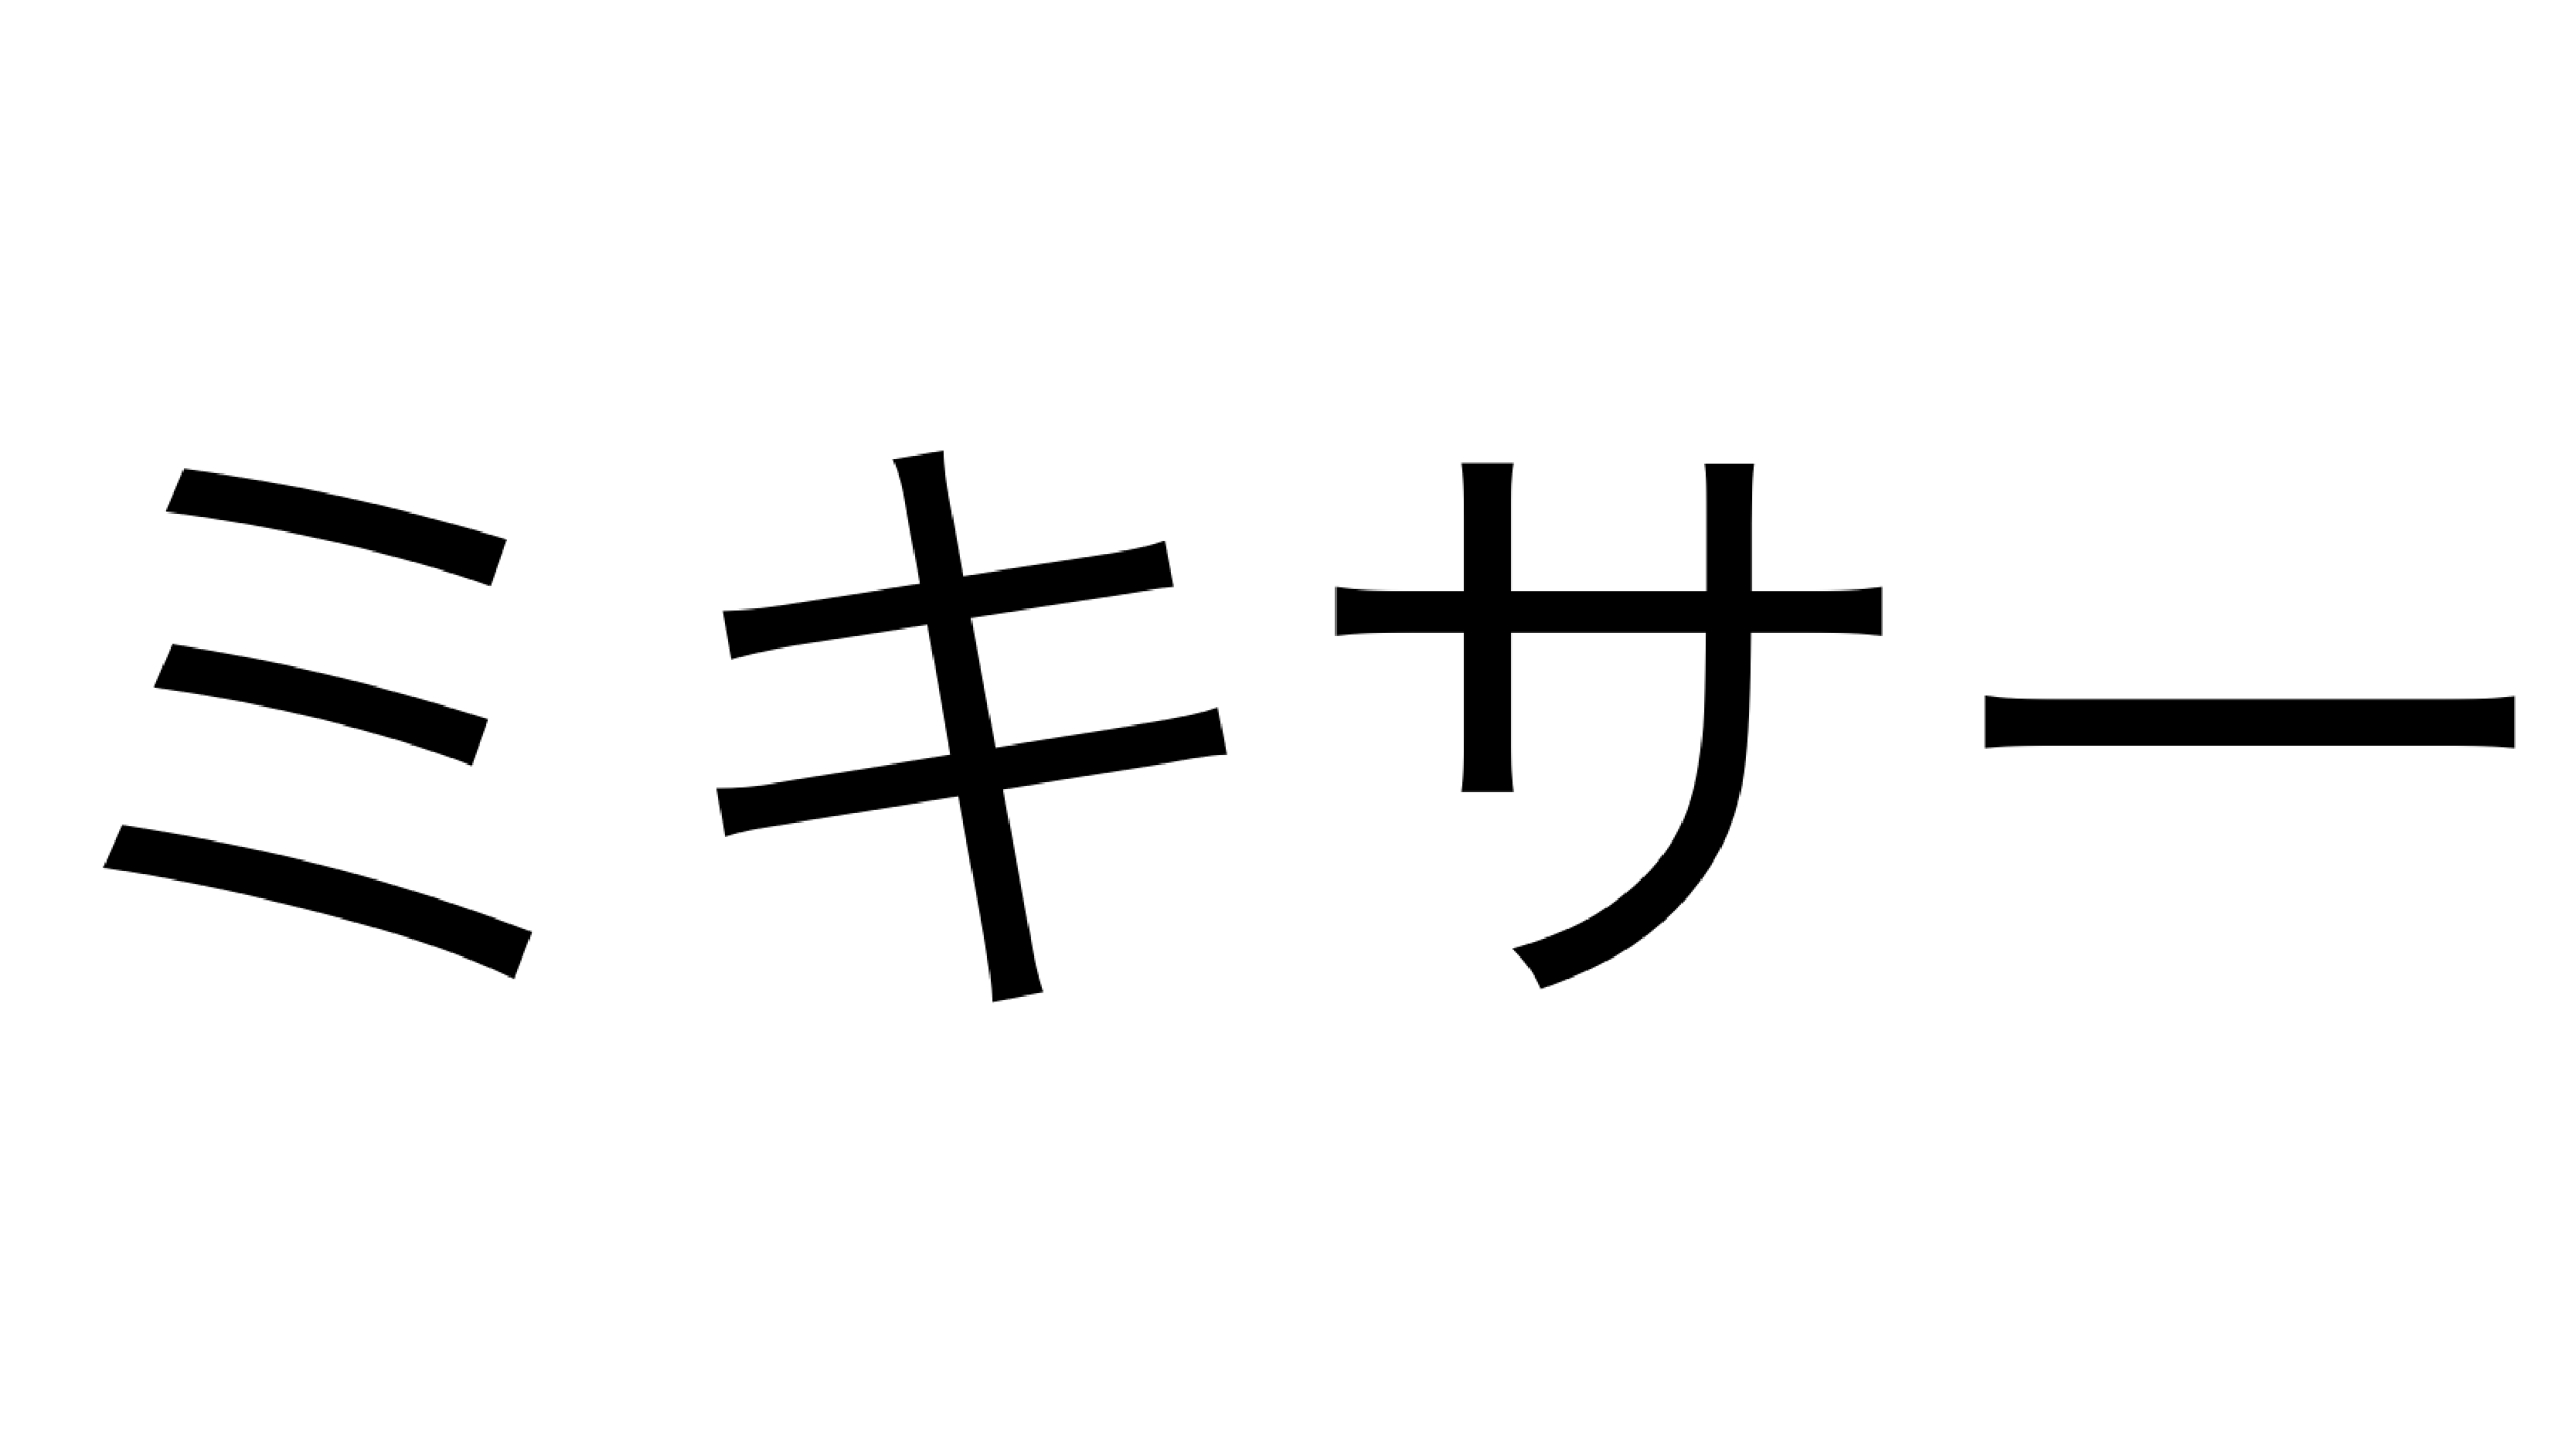
\includegraphics[width=0.4\linewidth]{img/mixer.pdf}
  \caption{ミキサー}
\end{figure}

\subsection{パワーアンプ}

ミキサーからの出力では、スピーカーを駆動させるのに必要な電気信号のレベルが不足している。電気信号を増幅させるのがパワーアンプと呼ばれる装置だ。ただし、スピーカーにパワーアンプが内蔵されているものもあり、その場合パワーアンプは不要となる。

\begin{figure}[htbp]
  \centering
  
\includegraphics[width=0.4\linewidth]{img/poweramp.pdf}
  \caption{パワーアンプ}
\end{figure}

\subsection{スピーカー}

スピーカーは、電気信号を音に変換する装置だ。人の耳に音を届けるために必要である。

\begin{figure}[htbp]
  \centering
  
\includegraphics[width=0.4\linewidth]{img/speaker.pdf}
  \caption{スピーカー}
\end{figure}

\subsection{映像機器}

オーディオ信号が、映像機器によって入力されることもある。たとえば、ビデオカメラの映像出力やPCの画面出力にオーディオ信号が入ることがある。ビデオスイッチャーによって映像・音声信号の分離が行われ、音声信号がミキサーに入力される構成が一般的だ。

\begin{figure}[htbp]
  \begin{minipage}{0.5\hsize}
    \centering
    
\includegraphics[width=\linewidth]{img/video_camera.pdf}
    \caption{ビデオカメラ}
  \end{minipage}
  \begin{minipage}{0.5\hsize}
    \centering
    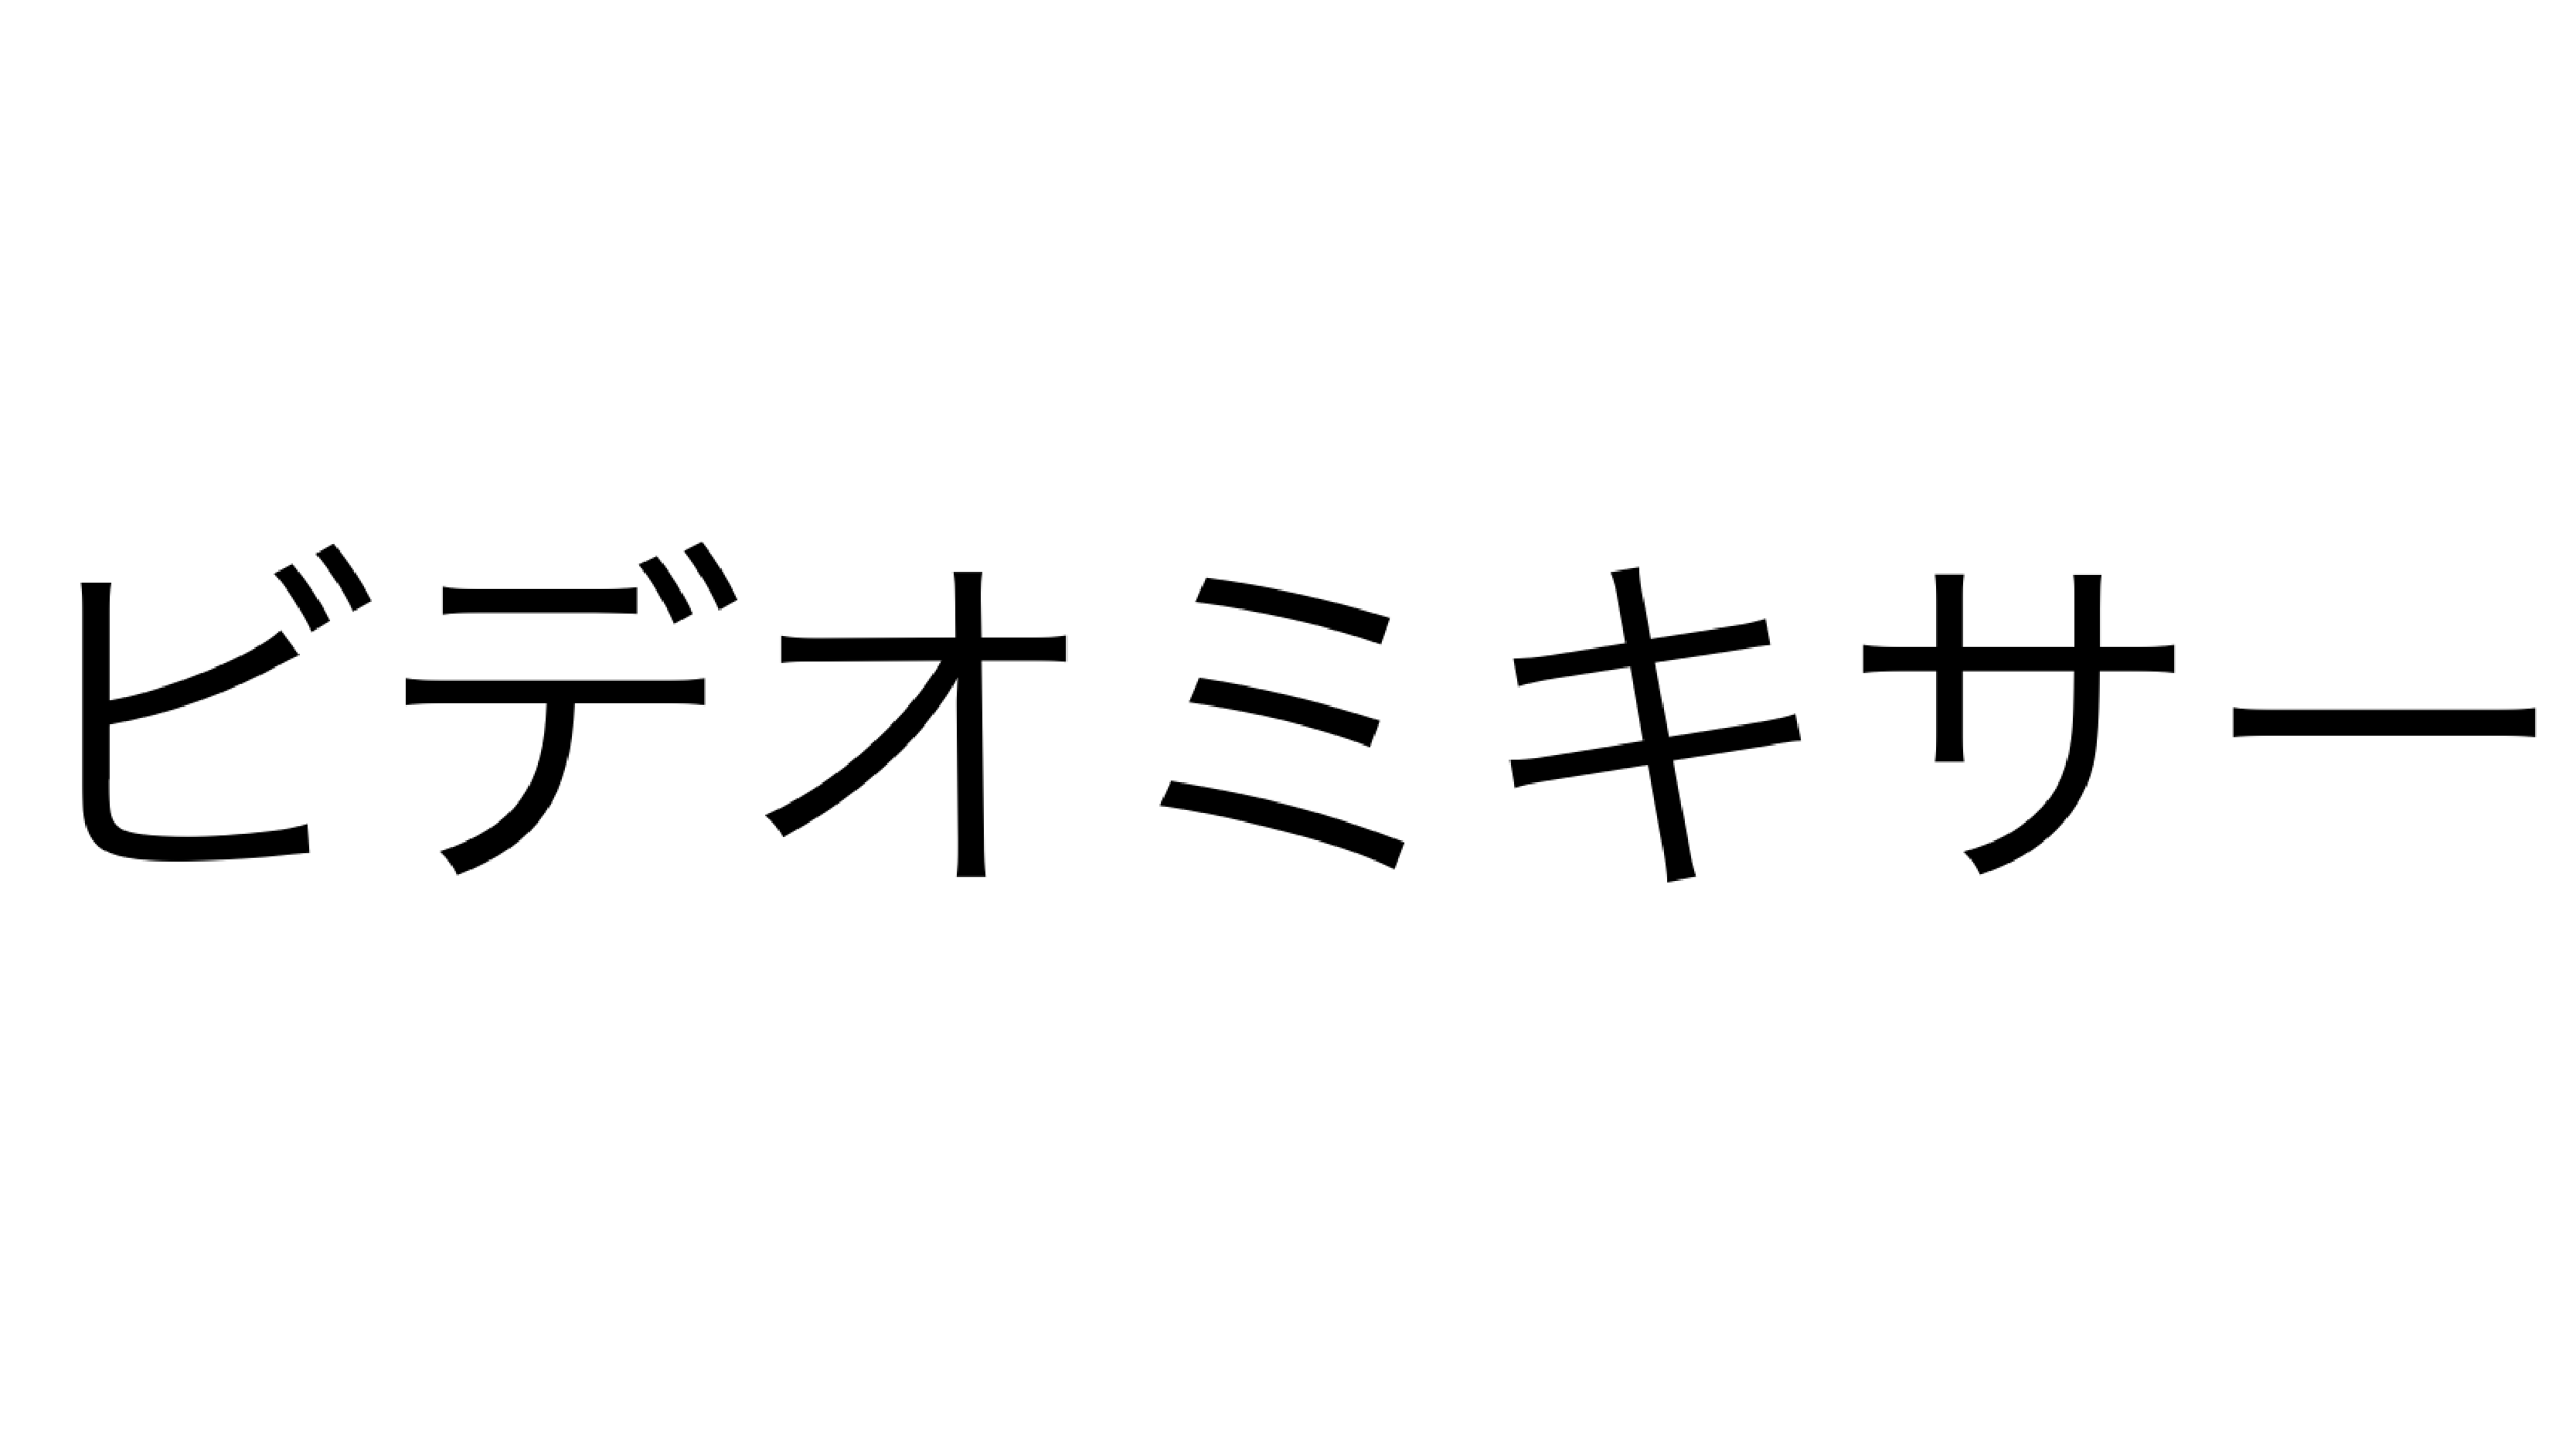
\includegraphics[width=\linewidth]{img/video_mixer.pdf}
    \caption{ビデオミキサー}
  \end{minipage}
\end{figure}

\section{インターフェイス}
\label{sec:interface}

\subsection{アナログ入出力}

うまい、やすい、はやい。

そんなうまい話は存在しない。

マルチケーブルを用いて1本で複数のチャンネルを束ねることもある。

\subsection{AES/EBU}
\label{sec:aes/ebu}

AES/EBUは、オーディオ専門家の国際組織である米国オーディオ技術者協会(AES)\footnote{Audio Engineering Society, Inc. \url{http://www.aes.org/}}と、欧州放送連合(EBU)\footnote{European Broadcasting Union \url{https://www.ebu.ch/home}}の両者によって策定されたデジタルオーディオ伝送規格である。それぞれAES3-1985\cite{aes3-1985}とEBU Tech.3250-E\cite{ebutech-3250-e}という名称で、1985年に策定された。なお、両者の名前をとって一般的にAES/EBUの名称で呼ばれている。

\subsubsection{IECによる標準化}

また、AES3は国際電気標準会議(IEC\footnote{International Electrotechnical Commission})によって標準化もされている。IECによる標準化では4つのパートで構成されており、IEC 60958-3ではAES3から派生した民生用途向け(いわゆるS/PDIF)と、IEC 60958-4ではAES3に基づいた業務用途向けのものが定められている。

接続するインターフェイスはIEC規格によって策定されている。アナログオーディオ伝送にも用いられるXLRコネクタによるバランス(平衡)接続や、BNCコネクタを用いた同軸ケーブルによるアンバランス(不平衡)接続、さらにはD-subコネクタを用いたオーディオ機器メーカーによる独自規格が存在する。本稿執筆時点で最新のAES3規格では、光ファイバーによる伝送も検討されている\footnote{AES3-2009 (r2019): AES standard for digital audio engineering - Serial transmission format for two-channel linearly represented digital audio data \url{http://www.aes.org/publications/standards/search.cfm?docID=13}}。

\subsubsection{AES-3id-1995}

BNCコネクタを用いたアンバランス接続は、AES3-id-1995という名称で策定されている。AES/EBUでは、インピーダンスが110Ωのケーブルを用いる。バランス接続は、ノイズの影響を受けにくく安定した伝送が期待できるものの、アンバランス接続の同軸ケーブルに比べ高価である。BNCコネクタが付いたインピーダンスが75Ωの同軸ケーブルは、業務用ビデオ伝送の分野で主流だ。

大規模なホールのような会場では予めさまざまな場所に配線しておき、パッチ盤で接続するという手法がある。パッチ盤のコネクタがBNCであれば何を伝送してもよいため、ビデオ伝送用に配線されている既存の同軸ケーブルを利用できる。AES/EBUで同軸ケーブルを用いて伝送するというアイデアは、ビデオ技術の団体米国映画テレビ技術者協会(SMPTE)\footnote{Society of Motion Picture and Television Engineers \url{https://www.smpte.org/}}からAESに対して要望が出ていたという経緯がある\cite{aes3id-1995-column}。同軸ケーブルを用いた伝送は、信号を補償(ブースト)することで長距離伝送が可能となる。同規格は、SMPTEからSMPTE 276M-1995という規格にもなっている。

\subsection{S/PDIF}

前述したとおり、業務用のAES/EBUから派生した民生用向けの規格は、IEC 60958-3によって標準化されている。この規格は、一般的にS/PDIF(Sony/Philips Digital Interface)と呼ばれる。日本のソニーとオランダのフィリップスが開発したためそのように呼ばれている。

AES/EBUでは、民生用では馴染みの薄いXLRコネクタやBNCコネクタが用いられてきたが、S/PDIFでは光デジタル音声端子(Optical)と同軸デジタル音声端子(Coaxial)の2種類が存在する。光デジタル端子は、東芝が提唱したTOSLINKと呼ばれる角型コネクタ、Mini-TOSLINKと呼ばれる3.5mmステレオミニプラグの形状をしたコネクタがある。同軸端子は、RCAコネクタが使われている。

Mini-TOSLINKは、以前AppleのパソコンであるiMacやMac mini、MacBook Proにも搭載されていた\footnote{MacBook Proは2015年発売の機種まで、3.5mmステレオミニジャックにアナログ入力とコンボジャックで搭載していた。 \url{https://support.apple.com/kb/SP719?locale=ja_JP&viewlocale=ja_JP}}。

\subsubsection{AES/EBUとS/PDIFの違い}

AES/EBUは業務用でS/PDIFは民生用だが、それぞれの違いを表\ref{tab:compare}に記す。業務用オーディオは、可能な限り伝送距離を長くし、XLRコネクタで接続した場合バランス接続による安定性をとっている。一方、民生用オーディオは出力レベルを低くし、伝送距離も10m程度である。ただし、著作権保護信号を伝送することができ、受信機が信号を認識するとその機器で録音ができなくなるようだ。

\begin{table}[htb]
  \begin{minipage}{\textwidth}
    \label{tab:compare}
    \caption{AES/EBUとS/PDIFの比較\cite{aesebuandspdif}}
    \begin{tabular}{c|ccc} \hline
      & AES3-1992 (r1997) & AES-3id-1995\footnote{SMPTE 276M-1995} & S/PDIF\footnote{IEC 60958-3} \\ \hline
      ケーブル & 110Ω STP & 75Ω 同軸 & 75Ω 同軸/光ファイバー \\
      インターフェイス & バランス & アンバランス & アンバランス \\
      コネクタ & 3ピンXLR & BNC & RCA / TOSLINK \\
      信号レベル & 2--7V peak to peak & 1.0--1.2V peak to peak & 0.5--0.6V peak to peak \\
      最小信号レベル & 0.2V & 0.32V & 0.2V \\
      最大伝送距離 & 100m & 1000m & 10m \\
      コピー制御 & 不可 & 不可 & 可能 \\
      ビット深度 & 24bit & 24bit & 20bit(24bitに拡張可能)\footnote{4bit分予備領域として確保されており、20+4bitを合わせて送信できる。} \\
    \end{tabular}
  \end{minipage}
\end{table}

\subsection{SDI}

SDI\footnote{Serial Digital Interface}は、ビデオ信号を伝送する規格である。非圧縮のビデオとオーディオを伝送することが可能だ。

本来はビデオ伝送用の規格だが、AES3に準拠した48kHz/24bitのオーディオを16チャンネル伝送できる。

\subsection{CobraNet}

CobraNetは、1996年に米Peak Audioが開発したEthernetを用いたオーディオ伝送規格である。Ethernetを使うが、IPベースでないのが特徴的だ\cite{best-practices-in-network-audio}。

\section{ケーブル}

\subsection{マイクケーブル}

さまざまなコネクタがあり、バランス接続ではXLR、TRS(モノラル)、アンバランス接続ではTRS(ステレオ)、RCAなどが存在する。コネクタを用いずに銅線そのままで接続する方法もある。

\subsection{スピーカーケーブル}
XLR、フォン、スピコン。パッシブスピーカーで使うが、パワードスピーカーはマイクケーブルで大丈夫。

\subsection{同軸ケーブル}

\subsection{光ケーブル}

\subsection{イーサネットケーブル}

\section{帯域}

民生用オーディオは圧縮されている場合がほとんど。MP3やAACオーディオはXXXkbps。一方、業務用オーディオは非圧縮のものが非常に多い。XXXMbpsほどで、圧倒的な情報量の存在。

\section{IPベースのデジタル伝送規格}

本項では、本研究と関連するオーディオのデジタル伝送を行う関連技術について、IPベースの伝送について示す。

\subsection{Internet Protocol}

\subsection{Ethernet AVB}

Ethernet AVBは、IEEE\footnote{Institute of Electrical and Electronics Engineers}により策定されたEthernetでオーディオとビデオを伝送する規格である。正式にはIEEE 802.1 Audio/Video Bridgingという。

\subsection{Dante}

Danteは、米Audinate\footnote{\url{https://www.audinate.com/?lang=ja}}が開発したIPベースのオーディオ伝送規格である。最大ビット深度は32bit、最大サンプリング周波数は192kHzで伝送できる\cite{best-practices-in-network-audio}。

2019年現在、ミキサーやパワーアンプなど、総合音響機器メーカーのヤマハや\footnote{\url{https://jp.yamaha.com/products/proaudio/index.html}}、パナソニック\footnote{\url{https://sol.panasonic.biz/sound/index.html}}、マイクメーカーの米Shure\footnote{\url{https://www.shure.com/ja-JP}}、独Sennheiser\footnote{\url{https://ja-jp.sennheiser.com/}}、オーディオテクニカ\footnote{\url{https://www.audio-technica.co.jp/proaudio/}}等のデジタルワイヤレスシステム、業務用レコーダー分野ではティアック(TASCAMブランド)\footnote{\url{https://tascam.jp/jp/}}など、幅広いメーカーと製品が対応しているAudio over IPのデファクトスタンダードともいえる規格だ。

\subsection{RAVENNA}

RAVENNA\footnote{\url{https://www.ravenna-network.com/}}は、独ALC NetworXが開発したIPベースのオーディオ伝送規格である。

他のIPベースの商用伝送規格と異なり、仕様がオープンになっておりRAVENNA Partner Networkとして各国のオーディオメーカーが参加している。

以下は、RAVENNAのWebサイト\footnote{"https://www.ravenna-network.com/about-ravenna/overview}に掲載されているRAVENNA Partner Networkに関する記述だ。

\begin{quotation}
  RAVENNA was developed by ALC NetworX who continues to be leading developer of the technology. However, given that RAVENNA is an open technology based on existing standards, this means that anyone is free to develop their own solutions. Indeed, this is actively encouraged in order to give customers as much choice as possible and not have to rely on ALC NetworX as the exclusive solution provider.
\end{quotation}

RAVENNAは、無償でバーチャルオーディオデバイスを公開している\footnote{\url{https://www.ravenna-network.com/resources/}}。Windows、macOS、Linuxに対応しており、インストールすることでRAVENNAとAES67機器とオーディオの送受信ができるようになる。

\subsection{AES67}

AES67は、AESが策定したIPベースのオーディオ伝送規格である。本研究において使用する規格でもある。\ref{sec:aes/ebu}節のAES/EBU同様、策定当初から仕様が公開されている。

DanteにはAES67 Modeオプションがあり、オプションを有効にすることでAES67対応機器とオーディオの送受信を行うことができる。RAVENNAにおいても、AES67に準拠して動作することが可能だ。AES67は、乱立するIPベースのオーディオ伝送規格を統一する目的で策定された。

AES67では、IP伝送においてマルチキャストとユニキャストをサポートしている。AES67で使用するIPバージョンはIPv4のみであり、IPv6はサポートされていない。しかしながら、将来IPv6をサポートする可能性を見据え、要所で対応のための準備が行われていることが仕様に書かれている。
